\documentclass[a4paper,11pt]{exam}
\printanswers % pour imprimer les réponses (corrigé)
%\noprintanswers % Pour ne pas imprimer les réponses (énoncé)
\addpoints % Pour compter les points
% \noaddpoints % pour ne pas compter les points
%\qformat{\textbf{\thequestion ) } }
\qformat{\textbf{\thequestion )}} % Pour définir le style des questions (facultatif)
\usepackage{color} % définit une nouvelle couleur
\shadedsolutions % définit le style des réponses
% \framedsolutions % définit le style des réponses
\definecolor{SolutionColor}{rgb}{0.8,0.9,1} % bleu ciel
\renewcommand{\solutiontitle}{\noindent\textbf{Solution:}\par\noindent} % Définit le titre des solutions




\makeatletter

\def\maketitle{{\centering%
	\par{\huge\textbf{\@title}}%
	\par{\@date}%
	\par}}


\renewcommand{\thesubsection}{\Alph{subsection}.}   

\makeatother

\lhead{NOM Pr\'enom :}
\rhead{\textbf{Les r\'eponses doivent \^etre justifi\'ees et r\'edig\'ees}}
\cfoot{\thepage / \pageref{LastPage}}


%\usepackage{../../pas-math}
%\usepackage{../../moncours}


%\usepackage{pas-cours}
%-------------------------------------------------------------------------------
%          -Packages nécessaires pour écrire en Français et en UTF8-
%-------------------------------------------------------------------------------
\usepackage[utf8]{inputenc}
\usepackage[frenchb]{babel}
%\usepackage{numprint}
\usepackage[T1]{fontenc}
%\usepackage{lmodern}
\usepackage{textcomp}
\usepackage[french, boxed]{algorithm2e}
\usepackage{hyperref}


%-------------------------------------------------------------------------------

%-------------------------------------------------------------------------------
%                          -Outils de mise en forme-
%-------------------------------------------------------------------------------
\usepackage{hyperref}
\hypersetup{pdfstartview=XYZ}
%\usepackage{enumerate}
\usepackage{graphicx}
\usepackage{multicol}
\usepackage{tabularx}
\usepackage{multirow}
\usepackage{color}
\usepackage{eurosym}


\usepackage{anysize} %%pour pouvoir mettre les marges qu'on veut
%\marginsize{2.5cm}{2.5cm}{2.5cm}{2.5cm}

\usepackage{indentfirst} %%pour que les premier paragraphes soient aussi indentés
\usepackage{verbatim}
\usepackage{enumitem}
\usepackage{booktabs}
\usepackage[usenames,dvipsnames,svgnames,table]{xcolor}

\usepackage{variations}

%-------------------------------------------------------------------------------


%-------------------------------------------------------------------------------
%                  -Nécessaires pour écrire des mathématiques-
%-------------------------------------------------------------------------------
\usepackage{amsfonts}
\usepackage{amssymb}
\usepackage{amsmath}
\usepackage{amsthm}
\usepackage{tikz}
\usepackage{xlop}
\usepackage[output-decimal-marker={,}]{siunitx}
%-------------------------------------------------------------------------------

%-------------------------------------------------------------------------------
%                  -Nécessaires pour écrire des formules chimiquess-
%-------------------------------------------------------------------------------

\usepackage[version=4]{mhchem}

%-------------------------------------------------------------------------------
% Pour pouvoir exploiter les fichiers directement dans beamer
\newcommand{\pause}{\ }
%-------------------------------------------------------------------------------
%                    - Mise en forme avancée
%-------------------------------------------------------------------------------

\usepackage{ifthen}
\usepackage{ifmtarg}


\newcommand{\ifTrue}[2]{\ifthenelse{\equal{#1}{true}}{#2}{$\qquad \qquad$}}

%\newcommand{\kword}[1]{\textcolor{red}{\underline{#1}}}
%-------------------------------------------------------------------------------

%-------------------------------------------------------------------------------
%                     -Mise en forme d'exercices-
%-------------------------------------------------------------------------------
%\newtheoremstyle{exostyle}
%{\topsep}% espace avant
%{\topsep}% espace apres
%{}% Police utilisee par le style de thm
%{}% Indentation (vide = aucune, \parindent = indentation paragraphe)
%{\bfseries}% Police du titre de thm
%{.}% Signe de ponctuation apres le titre du thm
%{ }% Espace apres le titre du thm (\newline = linebreak)
%{\thmname{#1}\thmnumber{ #2}\thmnote{. \normalfont{\textit{#3}}}}% composants du titre du thm : \thmname = nom du thm, \thmnumber = numéro du thm, \thmnote = sous-titre du thm

%\theoremstyle{exostyle}
%\newtheorem{exercice}{Exercice}
%
%\newenvironment{questions}{
%\begin{enumerate}[\hspace{12pt}\bfseries\itshape a.]}{\end{enumerate}
%} %mettre un 1 à la place du a si on veut des numéros au lieu de lettres pour les questions 
%-------------------------------------------------------------------------------

%-------------------------------------------------------------------------------
%                    - Mise en forme de tableaux -
%-------------------------------------------------------------------------------

\renewcommand{\arraystretch}{1.7}

\setlength{\tabcolsep}{1.2cm}

%-------------------------------------------------------------------------------



%-------------------------------------------------------------------------------
%                    - Racourcis d'écriture -
%-------------------------------------------------------------------------------
%Droites
\newcommand{\dte}[1]{$(#1)$}
\newcommand{\fig}[1]{figure $#1$}
\newcommand{\sym}{symétrique}
\newcommand{\syms}{symétriques}
\newcommand{\asym}{axe de symétrie}
\newcommand{\asyms}{axes de symétrie}
\newcommand{\seg}[1]{$[#1]$}
\newcommand{\monAngle}[1]{$\widehat{#1}$}
\newcommand{\bissec}{bissectrice}
\newcommand{\mediat}{médiatrice}
\newcommand{\ddte}[1]{$[#1)$}


% Angles orientés (couples de vecteurs)
\newcommand{\aopp}[2]{(\vec{#1}, \vec{#2})} %Les deuc vecteurs sont positifs
\newcommand{\aopn}[2]{(\vec{#1}, -\vec{#2})} %Le second vecteur est négatif
\newcommand{\aonp}[2]{(-\vec{#1}, \vec{#2})} %Le premier vecteur est négatif
\newcommand{\aonn}[2]{(-\vec{#1}, -\vec{#2})} %Les deux vecteurs sont négatifs

%Ensembles mathématiques
\newcommand{\naturels}{\mathbb{N}} %Nombres naturels
\newcommand{\relatifs}{\mathbb{Z}} %Nombres relatifs
\newcommand{\rationnels}{\mathbb{Q}} %Nombres rationnels
\newcommand{\reels}{\mathbb{R}} %Nombres réels
\newcommand{\complexes}{\mathbb{C}} %Nombres complexes


%Intégration des parenthèses aux cosinus
\newcommand{\cosP}[1]{\cos\left(#1\right)}
\newcommand{\sinP}[1]{\sin\left(#1\right)}


%Probas stats
\newcommand{\stat}{statistique}
\newcommand{\stats}{statistiques}


\newcommand{\homo}{homothétie}
\newcommand{\homos}{homothéties}


\newcommand{\mycoord}[3]{(\textcolor{red}{\num{#1}} ; \textcolor{Green}{\num{#2}} ; \textcolor{blue}{\num{#3}})}
%-------------------------------------------------------------------------------

%-------------------------------------------------------------------------------
%                    - Mise en page -
%-------------------------------------------------------------------------------

\newcommand{\twoCol}[1]{\begin{multicols}{2}#1\end{multicols}}


\setenumerate[1]{font=\bfseries,label=\textit{\alph*})}
\setenumerate[2]{font=\bfseries,label=\arabic*)}


%-------------------------------------------------------------------------------
%                    - Elements cours -
%-------------------------------------------------------------------------------

%Correction d'exercice
\newcommand{\exoSec}[2]{\subsection*{Exercice #1 page #2}}
%-------------------------------------------------------------------------------
%                    - raccourcis d'écriture -
%-------------------------------------------------------------------------------

%Mise en évidence de termes clés
\newcommand{\mykw}[1]{\textcolor{red}{\underline{\textbf{#1}}}}

%Exercices
\newcommand{\exo}[2]{exercice #1 page #2}
\newcommand{\Exo}[2]{Exercice #1 page #2}

\renewcommand{\pause}{\ }

%Intervalles
\newcommand{\interOO}[2]{$]$#1 , #2$[$}
\newcommand{\interOF}[2]{$]$#1 , #2$]$}
\newcommand{\interFO}[2]{$[$#1 , #2$[$}
\newcommand{\interFF}[2]{$[$#1 , #2$]$}



%\usepackage{fullpage}
\author{\ }
\date{22 Décembre 2017}
\title{Sciences Physiques : DS n° 3}


\begin{document}
%	\usepackage{fancyhdr}
%	
%	\pagestyle{fancy}
%	\fancyhf{}
	%\rhead{Share\LaTeX}

	\maketitle
\vspace*{-0.5cm}	

\begin{mydefs}
	\begin{itemize}
		\item \textbf{Satellite :} corps qui tourne autour d'une planète.
		\item \textbf{Orbite :} courbe décrite par un corps qui tourne autour d'un autre.
	\end{itemize}
\end{mydefs}
%\section{Définitions}


\begin{questions}
	\question Quelle est l'unité de mesure de l'intensité électrique ?
	\fillwithdottedlines{1cm}
	
	\question Quel appareil est utilisé pour mesurer la tension aux bornes d'un dipôle dans un circuit électrique, et comment est-il branché ?
	\fillwithdottedlines{1.5cm}

	\question Que dit la loi d'unicité de l'intensité électrique ?	
	\fillwithdottedlines{2cm}
%	\makeemptybox{5cm}
	
	
\end{questions}


\section{Convertir}

\begin{questions}
	\begin{multicols}{3}
		
	\question $\num{0.057} A = ................ mA$
	\question $\num{8.57} mA = ................ A$
	\question $\num{6} kA = ................ A$
	\question $\num{9521} mA = ................ kA$
	\question $\num{42.1} µA = ................ A$
	\question $\num{3.9} A = ................ mA$
	
	\end{multicols}
	
\end{questions}



\newpage 

%\section{Montage}

Jane a réalisé le circuit électrique ci-dessous :

\begin{center}
	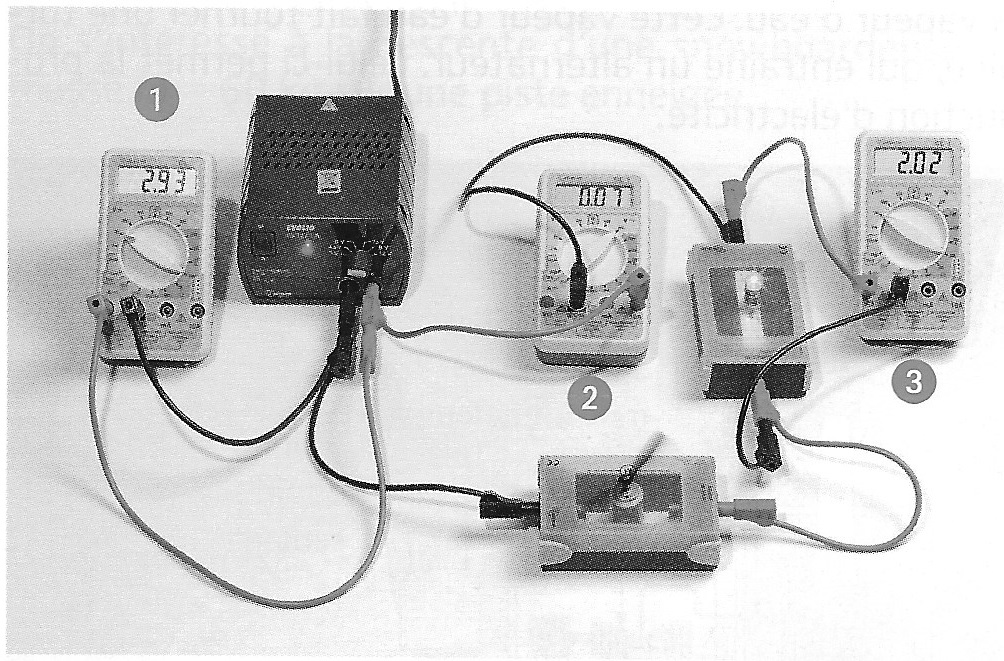
\includegraphics[scale=1.3]{img/montage_serie}
\end{center}

\begin{questions}
	
	\question 
		\begin{parts}
			\part Quels sont les appareils de mesure branchés en série ? en dérivation ?
			\fillwithdottedlines{2cm}
			\part Lesquels sont utilisés en voltmètre ? en ampèremètre ?
			\fillwithdottedlines{2cm}
		\end{parts}
	
	\question Réaliser le schéma normalisé du circuit de Jane.
	\makeemptybox{6.5cm}
	
	\question Quelles sont les tensions aux bornes :
	\begin{parts}
		\part du générateur ?
		\fillwithdottedlines{1.5cm}
		\part de la lampe ?
		\fillwithdottedlines{1.5cm}
		
		\part du moteur ?
		\fillwithdottedlines{1.5cm}
	\end{parts}

	\question Quelle est l'intensité du courant traversant :
	\begin{parts}
		\part la lampe ?
		\fillwithdottedlines{1.5cm}
		
		\part le moteur ?
		\fillwithdottedlines{1.5cm}
	\end{parts}

\end{questions}

\section{Montage}

Jane a réalisé le circuit électrique ci-dessous :

\begin{center}
	\includegraphics[scale=1]{img/montage_derivation2}
\end{center}

\begin{questions}
	
	\question 
	\begin{parts}
		\part Quels sont les appareils de mesure branchés en série ? en dérivation ?
		\fillwithdottedlines{2cm}
		\part Lesquels sont utilisés en voltmètre ? en ampèremètre ?
		\fillwithdottedlines{2cm}
	\end{parts}
	
	\question Réaliser le schéma normalisé du circuit de Jane.
	\makeemptybox{5.5cm}
	
	\question Quelles sont les tensions aux bornes :
	\begin{parts}
		\part du générateur ?
		\fillwithdottedlines{1.5cm}
		\part des lampes ?
		\fillwithdottedlines{1.5cm}
		
	\end{parts}
	
	\question Quelle est l'intensité du courant traversant :
	\begin{parts}
		\part les lampes $L_1$ et $L_2$ ?
		\fillwithdottedlines{1.5cm}
		
		\part le générateur ?
		\fillwithdottedlines{1.5cm}
	\end{parts}
	
\end{questions}

\section{Intensités manquantes}

Retrouver les valeurs des intensités du courant manquantes dans les circuits électriques ci-dessous. 

\begin{center}
	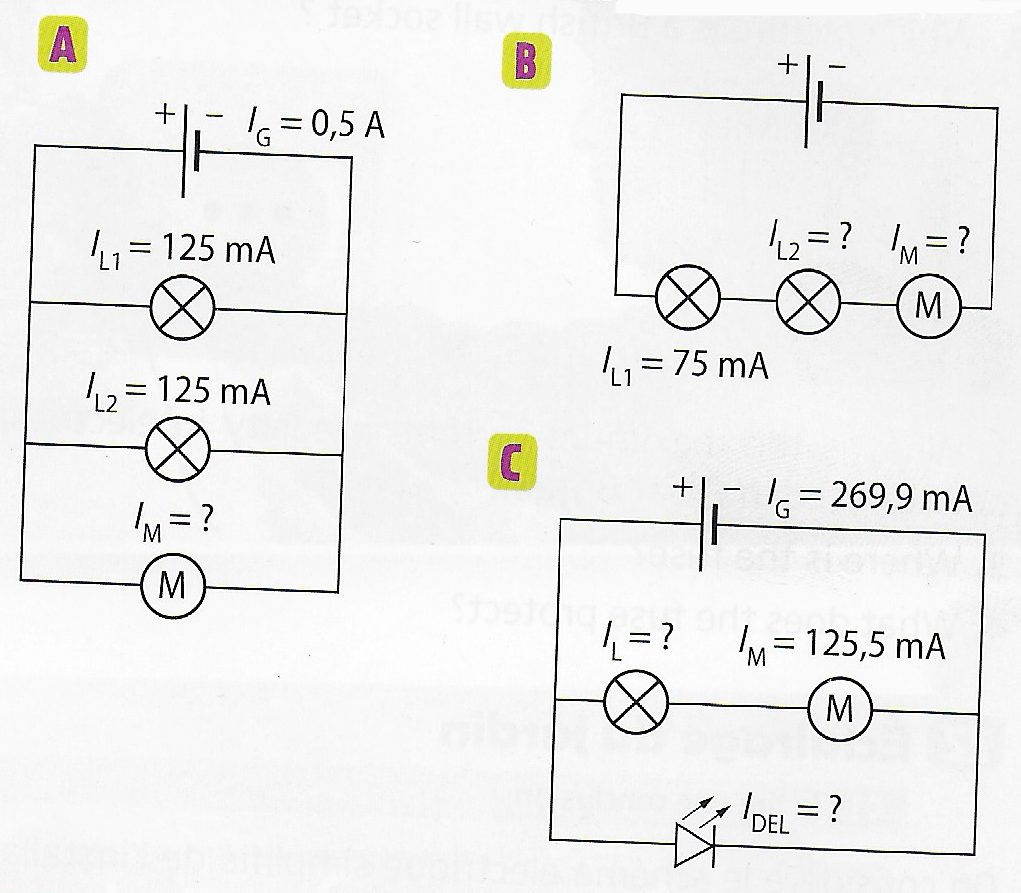
\includegraphics[scale=1]{img/circuits}
\end{center}


\fillwithdottedlines{4.5cm}



%\newpage

\section{\'Eclat des lampes}

Les lampes du circuit suivant sont toutes identiques. l'ampèremètre indique une intensité $I = \num{0.60} A.$

\begin{center}
	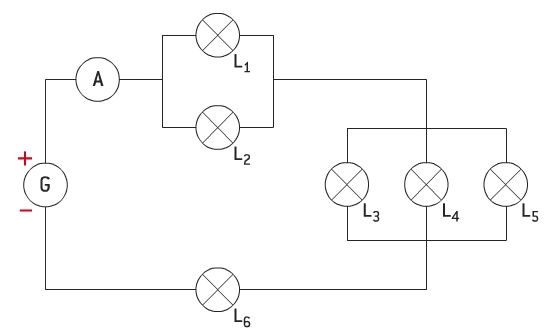
\includegraphics[scale=0.6]{img/ex_16}
\end{center}

\begin{questions}
	\question Quelle sera l'intensité du courant du courant circulant dans chaque lampe ?
	\fillwithdottedlines{3cm}
	
	\question Les lampes vont-elles briller de la même façon ?
	\fillwithdottedlines{2cm}
	
	\question Classer les lampes de celles qui ont l'éclat le plus fort à celles qui ont l'éclat le plus faible.
	\fillwithdottedlines{2cm}
	
\end{questions}




\ \label{LastPage}

\end{document}